% !TeX encoding = UTF-8
% !TeX spellcheck = russian-aot
% !TeX program = xelatex

\documentclass{article}

\usepackage[english, main=russian]{babel}
\usepackage{fontspec}
\setmainfont{Times New Roman}

\pagestyle{empty}

\usepackage[a5paper]{geometry}
\usepackage{pgfpages}
\pgfpagesuselayout{2 on 1}[a4paper, landscape, border shrink=5mm]

\usepackage{pgffor}

\usepackage{pdfpages}

\usepackage{hyperref}
\begin{document}

\begin{center}
	\Huge
	\vspace*\fill Оригинальный документ \vspace*\fill
	\newpage
	\vspace*\fill Документ мог бы выглядеть\vspace*\fill
\end{center}

	
\foreach \n in {1,2,3,4,5,6}{
	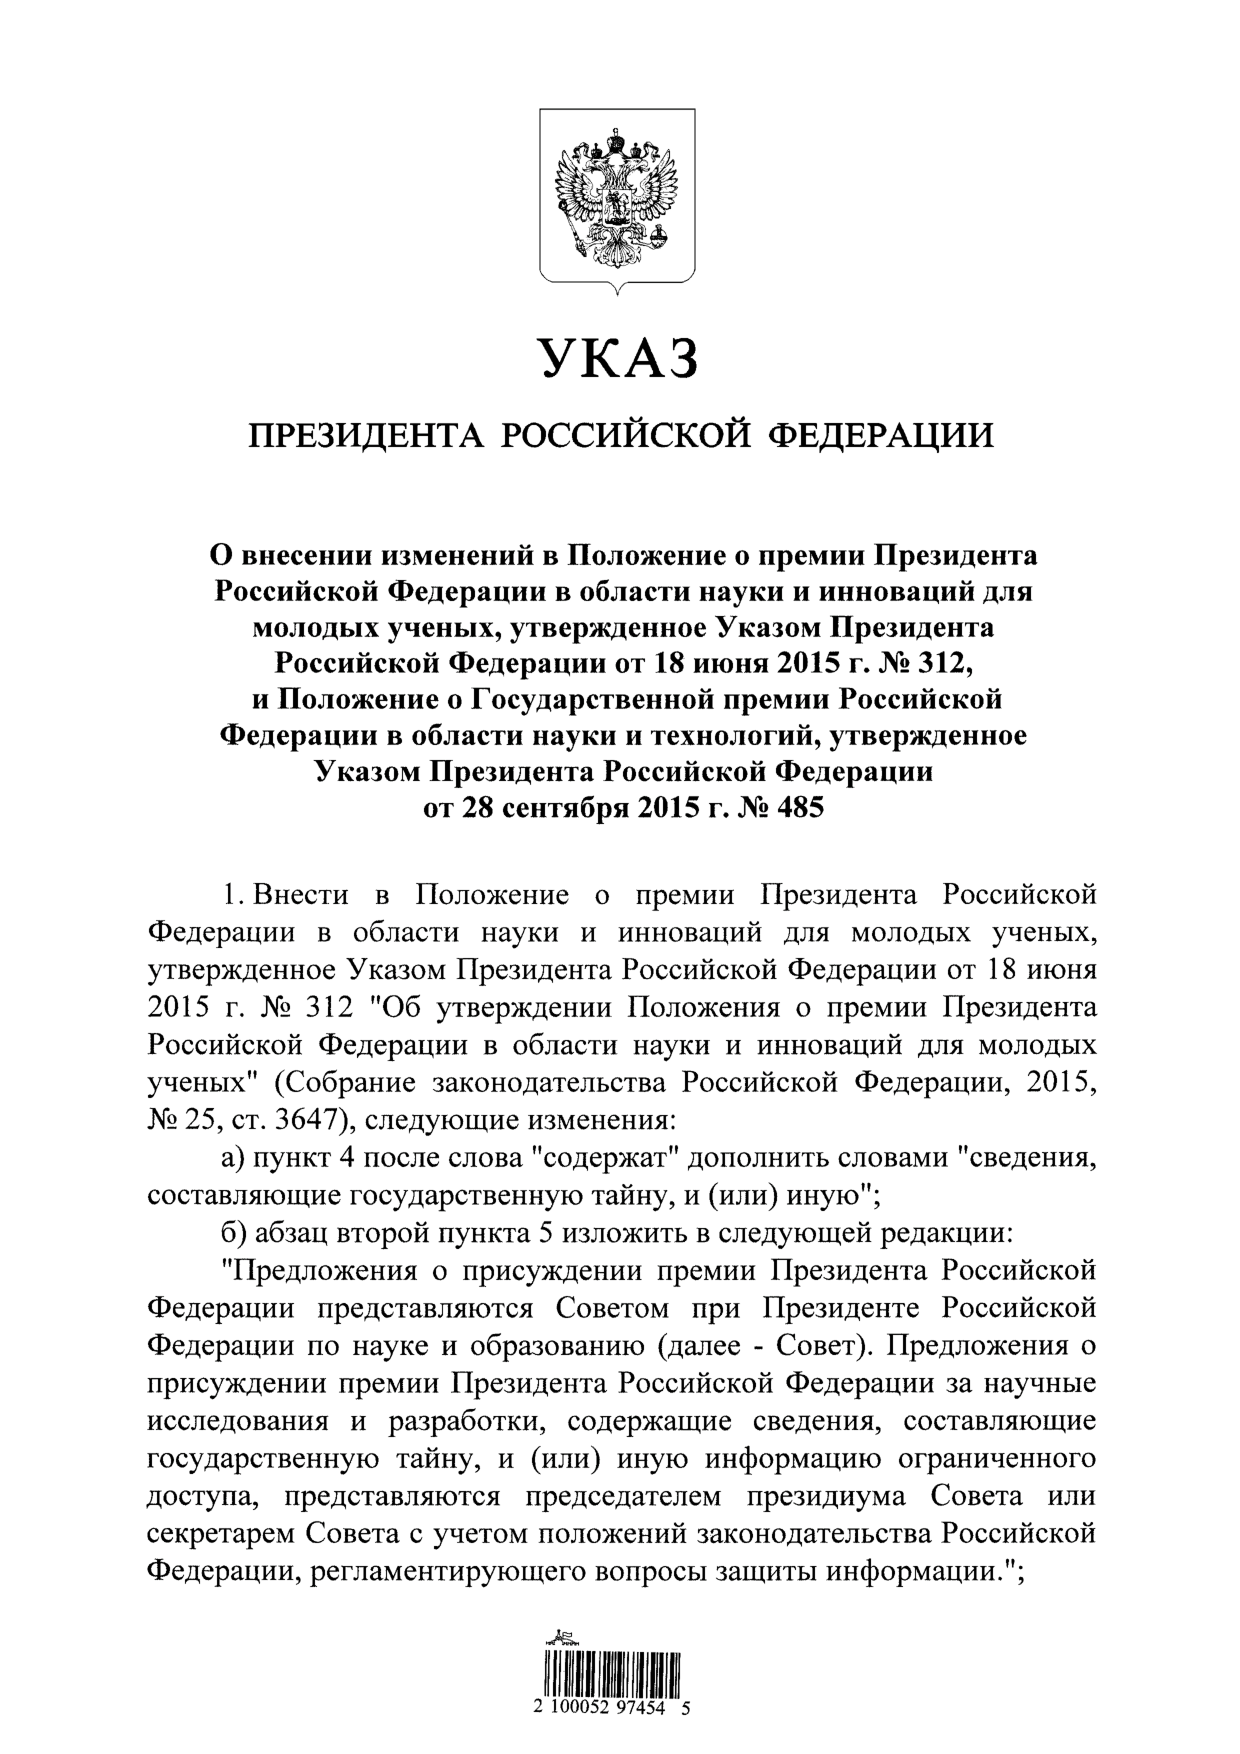
\includepdf[pages=\n, frame]{original.pdf}
	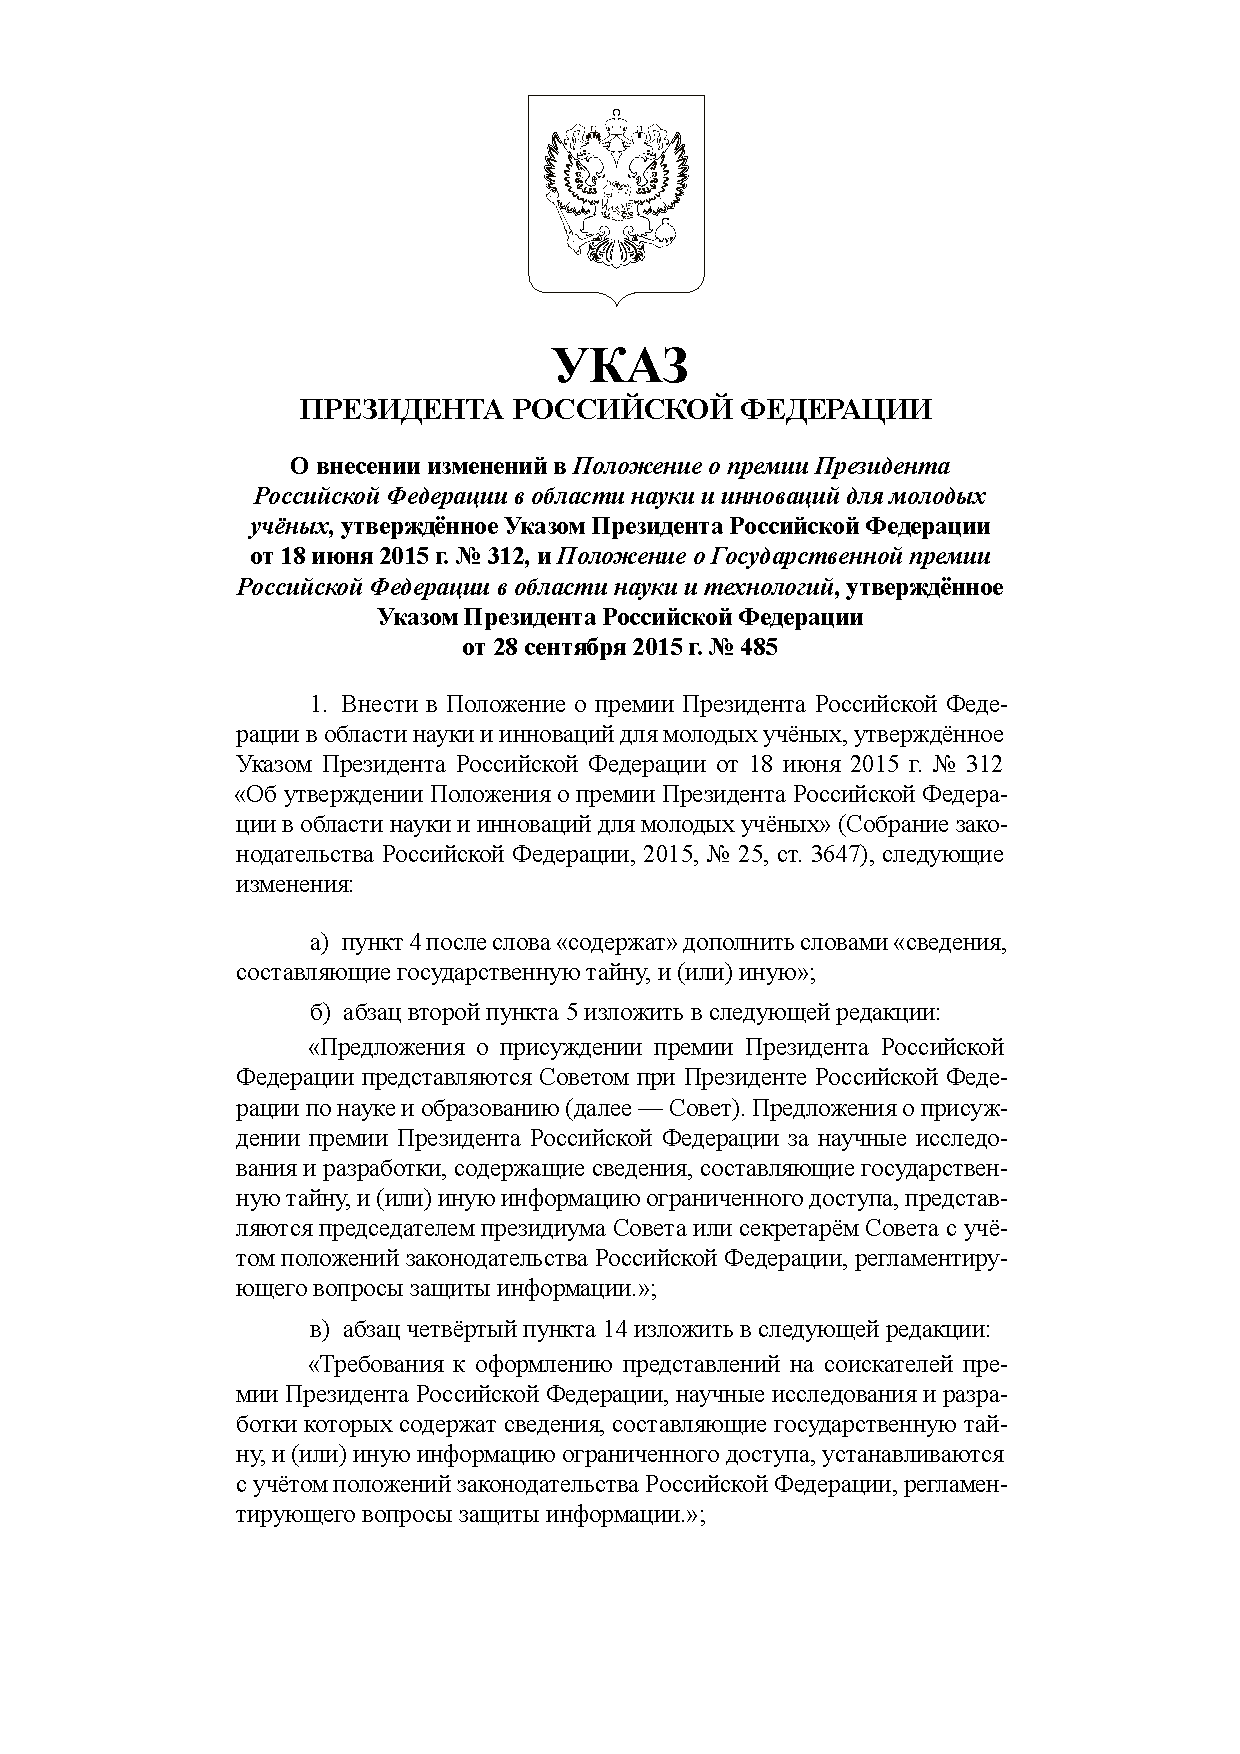
\includepdf[pages=\n, frame]{document.pdf}
}
\includepdf[pages=7, frame]{original.pdf}

\end{document}